\chapter{Introduction}

\section{Backgrounds}

This project, submitted to the \texttt{AI Builders X ESCK} program, originated from a series of questions.
\begin{itemize}
	\item What's the best way to blow on a liquid filled spoon to cool it?
	\item Given a room, what's the best place to place an air conditioner, and what direction must it face?
	\item What's the best place for a cooling fan in a CPU?,
\end{itemize}
etc. These problems are a set of problems that all fall in optimization problems in fluids:
\begin{quote}
	\emph{"Given an imposed boundary condition on a system containing fluids, a boundary condition that's free to move, and a certain function, find the boundary condition that optimizes the function."}
\end{quote}
E.g., in the first problem, the imposed boundary condition is the shape of the room; the free boundary condition is the placement and angle of the air conditioner, and the function is the time until the room reaches thermal equilibrium.

Due to the ten weeks time limit imposed by the \texttt{AI Builders X ESCK} program. We've decided to simplify various parts of the problem to make it more fathomable.

\section{Problem statement and overview of solution}

The problem that we've selected to tackle is the second problem due to phase homogeneity: \enquote{given a room, what's the best place to place an air conditioner, and what direction must it face.} Due to complexity in three-dimensions, we've decided to simplify the problem to a room with boundaries in two-dimensions, and only allow the air conditioner to exist on a line around the border of the room.

The variables that are used in this problem is as follows:
\begin{enumerate}[noitemsep]
	\item \textbf{The function needed for optimization}---the time until equilibrium
	\item \textbf{Free boundary condition}---placement of the air conditioner, represented as a density boundary condition
	\item \textbf{Imposed boundary condition}---shape of the room
\end{enumerate}
It's then solved as follows:
\begin{enumerate}[noitemsep]
	\item Build a fluid simulator with wall and density boundary condition,
	\item Input the shape of the room, and the strength of the air conditioner,
	\item Find the optimal air conditioner using gradient descent.
\end{enumerate}

Originally, we planned to use the \texttt{OpenFOAM} simulator, as it's commonly used by researchers in computational fluid dynamics. However, the learning curve is too steep for just ten weeks. There's no clean way to connect the data from \texttt{OpenFOAM} into \texttt{Python} for post-processing. Most importantly, there aren't many great resources out there. So, we've decided to build our own simulation and optimization algorithm from scratch using one of the most accessible methods to do fluid simulation: the Lattice-Boltzmann method.

\section{Overview of the Lattice-Boltzmann method}

The Lattice-Boltzmann method is a fluid simulation method that doesn't require discretization of the Navier-Stokes equation. Instead, it models fluids as a collection of particles in a lattice filled with cells. In each step of the simulation, the particle moves from its own cell to its adjacent cells. Then, it interacts inside the cell through self-collisions. This cell-interpretation allow the derivation of the macroscopic fluid properties, e.g., density and velocity, to be derived from the particle distributions in each lattice directly. The process includes
\begin{enumerate}
	\item \textbf{Streaming}---particles move into adjacent cells
	\item \textbf{Collisions}---the densities in each cell is adjusted towards equilibrium inside the cell.
\end{enumerate}

This method is very viable for parallel computing, making it very ideal for implementation in \texttt{NumPy}. However, it is numerically unstable for high-speed fluid flows near or above the speed of sound. Since we're not dealing with particles moving that fast, we should be fine.

Even though the Lattice-Boltzmann method is stable for the most part, it still has some numerical instabilities around boundary conditions especially anything to do with circles. These will become a problem in gradient descent, in which we have to implement an algorithm to work around these instabilities.

\subsection{Representation}

\paragraph{Coordinate convention} Since \texttt{NumPy} indexes the $y$-axis (vertically) before the $x$-axis (horizontally), all pairs of coordinates from now on is to be read as $(y, x)$, not $(x, y)$

A fluid simulation with resolution $N \times M$ illustrated in \cref{fig:fluid-lattice}, is represented as a rectangular lattice with $N \times M$ cells. Each cell in the lattice contains nine cell-invariant unit vectors, $\vv{e}_0$ to $\vv{e}_8$, which represents the eight possible direction that the fluid can travel in. The value for these vectors, respective to the Cartesian representation is given in \cref{tab:unit-vectors}

\begin{table}[ht]
	\centering
	\begin{tabular}{C | C}
		\textrm{Unit vector} & \textrm{Representation} \\
		\hline
		\vv{e}_0             & \vv{0}                  \\
		\vv{e}_1             & \xhat                   \\
		\vv{e}_2             & \yhat                   \\
		\vv{e}_3             & -\xhat                  \\
		\vv{e}_4             & -\yhat                  \\
		\vv{e}_5             & \xhat + \yhat           \\
		\vv{e}_6             & -\xhat + \yhat          \\
		\vv{e}_7             & -\xhat - \yhat          \\
		\vv{e}_8             & \xhat - \yhat
	\end{tabular}
	\caption{Unit vectors used in a cell of fluid}
	\label{tab:unit-vectors}
\end{table}

\begin{figure}[ht]
	\centering
	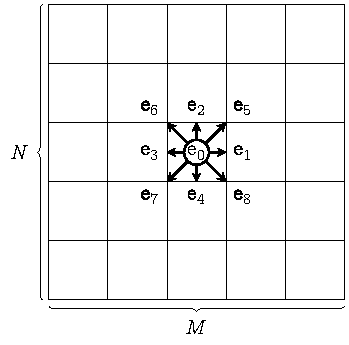
\includegraphics{fluid-lattice.pdf}
	\caption{Lattice of fluid}
	\label{fig:fluid-lattice}
\end{figure}

From the set of vectors $\vv{e}_0, \dots, \vv{e}_8$ inside each cell, one respectively assign another set of vectors $\vv{f}_0, \dots, \vv{f}_8$. These vectors are scaled version of the unit vectors, i.e.,
\begin{equation}
	\vv{f}_i = f_i\vv{e}_i,
\end{equation}
where the scalar $f_n$ represents the amount of fluid that's moving in the direction $\vv{e}_n$. From this representation alone, the density, momentum, and speed of the fluid at a certain point $(n, m)$ can be found. The density of fluid at the cell $(n, m)$, $\rho(n, m)$, is the sum from of all $f_i$'s inside the cell:
\begin{equation}
	\rho(n, m) \equiv \sum_if_i(n, m). \label{eq:density-calculation}
\end{equation}
The momentum density, $\vv{U}(n, m)$, traditionally given by the product between velocity and mass, can be calculated as the sum of product between $f_n$ and their respective unit vectors:
\begin{equation}
	\vv{U}(n, m) \equiv \sum_nf_n\vv{e}_n. \label{eq:momentum-calculation}
\end{equation}
The velocity density at a certain cell is just the ratio between the momentum density and the fluid density:
\begin{equation}
	\vv{u}(n, m) \equiv \frac{\vv{U}(n, m)}{\rho(n, m)} = \frac{\sum_nf_n\vv{e}_n}{\rho}. \label{eq:velocity-calculation}
\end{equation}

\subsection{Self-collision step}

The self-collision step represents the relaxation of fluid that happens inside a cell. In each of the fluid vectors $\vv{f}_0,\dots,\vv{f}_8$, a corresponding equilibrium vector is assigned by
\begin{equation}
	\vv{E}_i(n, m) = w_i\rho\ab(1 + 3\vv{e}_i \cdot \vv{u}(n, m) + \frac{9}{2}\ab(\vv{e}_i \cdot \vv{u}(n, m))^2 - \frac{3}{2}|\vv{u}(n, m)|^2)\vv{e}_i \label{eq:self-collision-calculation-1}
\end{equation}
where $w_i$ is a weighting factor that's given by the reduction of Boltzmann's distribution:
\begin{gather}
	w_i = \begin{cases}
		\frac{4}{9}  & \textrm{if} ~ i = 0,          \\
		\frac{1}{9}  & \textrm{if} ~ i = 1, 2, 3, 4, \\
		\frac{1}{36} & \textrm{if} ~ i = 5, 6, 7, 8.
	\end{cases} \label{eq:lbm-weights}
\end{gather}
The corresponding equilibrium scalar $E_i(n, m)$, is given by the relation
\begin{equation}
	\vv{E}_i(n, m) = E_i(n, m)\vv{e}_i.
\end{equation}

However, a fluid cannot possibly reach its own equilibrium in just one step; therefore, the Lattice-Boltzmann adjusts the fluid vector to approach the equilibrium vector. This behavior is captured by the relaxation time $\tau$. For the set of fluid vector positioned at the cell $(n, m)$ at time $t$, $f_i(n, m; t)$, the fluid vector at the next time step, $t + \Dd{t}$ is given by
\begin{equation}
	f_i(n, m; t + \Dd{t}) = f_i(n, m; t) + \frac{1}{\tau}\ab(E_i(n, m; t) - f_i(n, m; t)), \label{eq:self-collision-calculation-2}
\end{equation}
and that
\begin{equation}
	\vv{f}_i(n, m; t + \Dd{t}) = f_i(n, m; t + \Dd{t})\vv{e}_i.
\end{equation}

The relaxation value that's used throughout this project is $\tau = 0.8070$, which is said to be the most numerically stable \cite{zhao-2013}.

\subsection{Streaming step}

Using the vector that's adjusted to the equilibrium from the self-collision step, that vector is streamed to the adjacent cells, given by
\begin{equation}
	\vv{f}_i\ab(n + (\yhat \vdot \vv{e}_i), m + (\xhat \vdot \vv{e}_i)) = \vv{f}_i(n, m; t + \Dd{t}).
\end{equation}
Basically, this equation moves the fluid from one cell to the other as illustrated in \cref{fig:streaming-step}
\begin{figure}
	\centering
	\begin{subfigure}{0.45\textwidth}
		\centering
		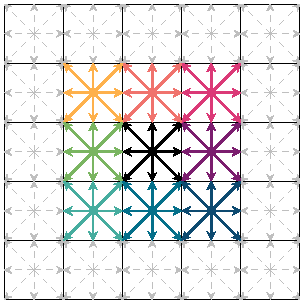
\includegraphics{streaming-before.pdf}
		\caption{Before}
	\end{subfigure}
	\begin{subfigure}{0.45\textwidth}
		\centering
		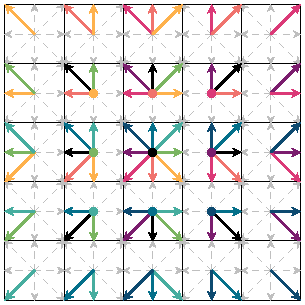
\includegraphics{streaming-after.pdf}
		\caption{After}
	\end{subfigure}
	\caption{Fluid vectors before and after the streaming step highlighted in color. Gray vectors are not considered.}
	\label{fig:streaming-step}
\end{figure}

\subsection{Boundary conditions}

There are two boundaries condition that needs to be implemented in this problem: wall and density. Since we want this to be a complete framework for two-dimensional fluid simulation, we also implemented the density boundary condition for completeness' sake.

\paragraph{Directional density boundary condition} This boundary condition can be achieved by explicitly setting the value of $f_0$ to $f_8$ after a complete simulation step.

\paragraph{Wall boundary condition} This boundary condition is sometimes referred off as the bounce-back boundary condition. If the fluid from an adjacent cell is streamed into a wall located at $(n, m)$, the wall simply reflects the fluid vector back:
\begin{equation}
	f_j\ab(n - (\vv{e}_i \vdot \yhat), m - (\vv{e}_i \vdot \xhat)) = f_i(n, m) \label{eq:wall-boundary-calculation}
\end{equation}
where
\begin{equation}
	j = \begin{cases}
		i + 2 & \textrm{if} ~ i = 1, 2, 5, 6, \\
		i - 2 & \textrm{if} ~ i = 3, 4, 7, 8.
	\end{cases} \label{eq:wall-boundary-calculation-relation}
\end{equation}
Since the fluid cannot possibly stream into the center of the wall, $j$ doesn't have to be defined at $i = 0$. \cite{adams-no-date}

\paragraph{Wall-velocity boundary condition} Given a wall that's located at position $(n, m)$, and an exposed fluid cell located at position $\ab(n + (\vv{e}_a\vdot\yhat), m + (\vv{e}_b\vdot\xhat))$, the velocity boundary condition can be defined by two variables: velocity along $\vv{e}_a$, and along its clockwise perpendicular, $\vv{e}_b$ where
\begin{equation}
	b = \begin{cases}
		a + 3 & \textrm{if} ~ a = 1,       \\
		a - 1 & \textrm{if} ~ a + 2, 3, 4.
	\end{cases}
\end{equation}
Here, we define the other directions that are relative to direction $a$:
\begin{gather}
	\alpha = \begin{cases}
		a + 2 & \textrm{if} ~ a = 1, 2, \\
		a - 2 & \textrm{if} ~ a = 3, 4,
	\end{cases} \\
	\beta = \begin{cases}
		a + 1 & \textrm{if} ~ a = 1, 2, 3, \\
		a - 3 & \textrm{if} ~ a = 4,
	\end{cases} \\
	A = \begin{cases}
		a + 7 & \textrm{if} ~ a = 1,       \\
		a + 3 & \textrm{if} ~ a = 2, 3, 4,
	\end{cases} \\
	B = \begin{cases}
		a + 6 & \textrm{if} ~ a = 1, 2, \\
		a + 2 & \textrm{if} ~ a = 3, 4,
	\end{cases} \\
	C = \begin{cases}
		a + 5 & \textrm{if} ~ a = 1, 2, 3, \\
		a - 1 & \textrm{if} ~ a = 4,
	\end{cases} \\
	D = a + 4.
\end{gather}
These directions live on a grid relative to direction $a$ as illustrated in \cref{fig:relative-direction}.
\begin{figure}[ht]
	\centering
	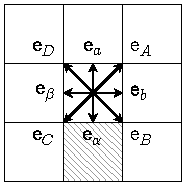
\includegraphics{relative-direction.pdf}
	\caption{Directions relative to the convention given by the wall-velocity boundary condition. The shaded region is the wall, and the cell with vector arrows is the target cell in which wall-velocity boundary condition is applied.}
	\label{fig:relative-direction}
\end{figure}
\begin{table}[ht]
	\centering
	\begin{tabular}{C C | C C C C C C}
		a & b & \alpha & \beta & A & B & C & D \\
		\hline
		1 & 4 & 3      & 2     & 8 & 7 & 6 & 5 \\
		2 & 1 & 4      & 3     & 5 & 8 & 7 & 6 \\
		3 & 2 & 1      & 4     & 6 & 5 & 8 & 7 \\
		4 & 3 & 2      & 1     & 7 & 6 & 5 & 8
	\end{tabular}
	\caption{Directions relative to the convention given by the wall-velocity boundary condition.}
	\label{tab:relative-direction}
\end{table}

Given that
\begin{equation}
	\vv{u}_a\ab(n + (\vv{e}_a\vdot\yhat), m + (\vv{e}_b\vdot\xhat)) \mathand \vv{u}_b\ab(n + (\vv{e}_a\vdot\yhat), m + (\vv{e}_b\vdot\xhat))
\end{equation}
is fixed by the boundary condition, the surrounding velocities in the cell $\ab(n + (\vv{e}_a\vdot\yhat), m + (\vv{e}_b\vdot\xhat))$ can be updated as follows: \cite{zou-1997}
\begin{gather}
	\vv{f}_a = \vv{f}_{\alpha} + \frac{2}{3}\rho\ab(n + (\vv{e}_a\vdot\yhat), m + (\vv{e}_b\vdot\xhat))\vv{f}_a, \label{eq:velocity-boundary-1} \\
	\vv{f}_A = \vv{f}_{C} - \frac{1}{2}\ab(\vv{f}_b - \vv{f}_{\beta}) + \rho\ab(n + (\vv{e}_a\vdot\yhat), m + (\vv{e}_b\vdot\xhat))\ab(\frac{\vv{u}_b}{6} + \frac{\vv{u}_a}{6}), \label{eq:velocity-boundary-2}\\
	\vv{f}_D = \vv{f}_{B} - \frac{1}{2}\ab(\vv{f}_b - \vv{f}_{\beta}) + \rho\ab(n + (\vv{e}_a\vdot\yhat), m + (\vv{e}_b\vdot\xhat))\ab(- \frac{\vv{u}_b}{6} + \frac{\vv{u}_a}{6}). \label{eq:velocity-boundary-3}
\end{gather}
For the rest of the directions, use the wall boundary condition (bounce-back) to calculate the fluids vector.
